% Source: src-b19b233abb266d1b051ded3c332a399c1722d8192d07ce1bf2234dda57bd25bc, PDF p.4.
% Cone topology and parallel OC/SD relation; projection is schematic, not metric.
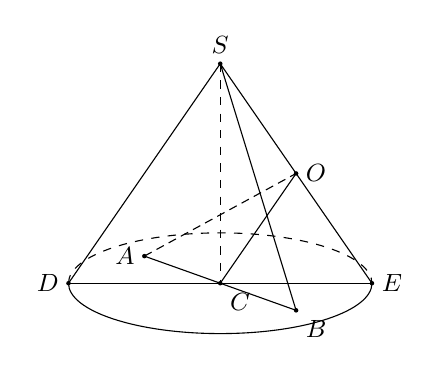
\begin{tikzpicture}[scale=0.82, every node/.style={font=\small}]
  \coordinate (S) at (0,3.4);
  \coordinate (D) at (-2.35,0);
  \coordinate (E) at (2.35,0);
  \coordinate (C) at (0,0);
  \coordinate (A) at (-1.175,0.42);
  \coordinate (B) at (1.175,-0.42);
  \coordinate (O) at (1.175,1.7);
  \draw (S)--(D) (S)--(E) (S)--(B);
  \draw[dashed] (S)--(C);
  \draw (D) arc[start angle=180,end angle=360,x radius=2.35,y radius=0.78];
  \draw[dashed] (D) arc[start angle=180,end angle=0,x radius=2.35,y radius=0.78];
  \draw (D)--(E);
  \draw (A)--(B);
  \draw (C)--(O);
  \draw[densely dashed] (A)--(O);
  \fill (S) circle (1pt);
  \fill (D) circle (1pt);
  \fill (E) circle (1pt);
  \fill (A) circle (1pt);
  \fill (B) circle (1pt);
  \fill (C) circle (1pt);
  \fill (O) circle (1pt);
  \node[above] at (S) {$S$};
  \node[left] at (D) {$D$};
  \node[right] at (E) {$E$};
  \node[left] at (A) {$A$};
  \node[below right] at (B) {$B$};
  \node[below right] at (C) {$C$};
  \node[right] at (O) {$O$};
\end{tikzpicture}
